\documentclass[12pt]{article}

\usepackage{tabularx}
\usepackage[a4paper,margin=2.5cm, bottom=3.5cm]{geometry}
\usepackage{fancyhdr}
\usepackage{listings}
\usepackage{booktabs}
\usepackage{float}
\usepackage{subcaption}
\usepackage{graphicx}
\usepackage{amsmath}
\usepackage{amssymb}
\usepackage{amsthm}
\usepackage{array}
\usepackage[table]{xcolor}
\usepackage{pgfplots}
\usepackage{pgfplotstable}
\usepackage{multirow}
\usepackage{tikz}
\usepackage[hidelinks]{hyperref}
\usepackage{titling}
\pgfplotsset{compat=1.17}

\theoremstyle{definition}
\newtheorem*{example}{Example}
\setlength{\headheight}{40pt}
\setlength{\parindent}{0pt}
\setlength{\parskip}{1ex}
\renewcommand{\headrulewidth}{0pt}

\newcommand{\subfiguresize}{.3\textwidth}
\DeclareMathOperator*{\median}{median}

\DeclareMathOperator*{\biggerforall}{\mbox{\Large $\mathsurround0pt\forall$}} 
\DeclareMathOperator*{\bigforall}{\mbox{\large $\mathsurround0pt\forall$}} 
\DeclareMathOperator*{\biggerexists}{\mbox{\Large $\mathsurround0pt\exists$}} 
\DeclareMathOperator*{\bigexists}{\mbox{\large $\mathsurround0pt\exists$}} 

\lstset {
    captionpos = b,
    basicstyle = \small\ttfamily,
    keywordstyle = \color{blue},
    commentstyle = \color{black!30},
    comment = [l]{//},
    morecomment = [s]{/*}{*/},
    identifierstyle=,
    keywords = {
        let,
        mut,
        for,
        in,
        if,
        else,
        continue,
        break,
        pub,
        struct,
        impl,
        type,
        self,
        Self,
        as,
        u8,u16,u32,u64,
        i8,i16,i32,i64,
        f32,f64,
        usize,
    }
}

\pagestyle{fancy}
\fancyhead{}
\fancyhead[L]{
    \renewcommand{\arraystretch}{1.5}
    \begin{tabularx}{\textwidth}{|X|X|}
        \hline
        \large \bf Image processing & \normalsize \thetitle \\
        \hline
    \end{tabularx}
}
\fancyfoot[C]{\thepage}

\renewcommand{\maketitle}{
    \thispagestyle{plain}
    \renewcommand{\arraystretch}{2}
    \vspace*{-7em}
    \begin{flushleft}
        \begin{tabularx}{0.95\textwidth}{|X|X|}
            \hline
            \bf \large Image Processing                   & \bf \large \thetitle                           \\ \hline
            \multicolumn{2}{|l|}{
                \textbf{Task variant:} Group 1
            }                                                                                               \\ \hline
            \textbf{Day and time:} Mon, 14:00             & \textbf{Full name:} \textsc{Jakub Pawlak}       \\
            \textbf{Academic year:} {2022/23} & \textbf{Full name:} \textsc{Magdalena Paku\l a} \\
            \hline
        \end{tabularx}
    \end{flushleft}
    \vspace{1em}
    \renewcommand{\arraystretch}{1}
}
\graphicspath{{img},{../img}}

\newcommand*{\fft}{\textsc{fft}}
\newcommand*{\dft}{\textsc{dft}}

\title{Task No.~4}

\begin{document}

\maketitle

\section{Description of the implementation of the assigned transform variant}

We decided to implement the \fft\ using the radix-2 decimation in time variant of the Cooley-Turkey algorithm.
It uses the divide-and-conquer approach to divide a \dft\ of length $N$ into two \dft{}s of length $\frac{N}{2}$.
The speed is gained by reusing some computations for multiple \dft\ outputs.

\begin{figure}[H]\centering
    \begin{tikzpicture}
        \foreach \i in {0,...,7} {
                \node[circle, draw=black, inner sep=0pt, minimum size=2pt](start-\i) at (0,-\i) {};
                \draw[-latex] (start-\i) -- (1,-\i);
                \draw(1,-\i) -- (2,-\i);
            }
        \draw (0, 0) node[left]{$x[0]$};
        \draw (0,-1) node[left]{$x[2]$};
        \draw (0,-2) node[left]{$x[4]$};
        \draw (0,-3) node[left]{$x[6]$};

        \draw (0,-4) node[left]{$x[1]$};
        \draw (0,-5) node[left]{$x[3]$};
        \draw (0,-6) node[left]{$x[5]$};
        \draw (0,-7) node[left]{$x[7]$};

        \draw (2, 0.25) -| ++(2, -3.5) -| cycle;
        \draw (2,-3.75) -| ++(2, -3.5) -| cycle;

        \draw (3,-1.5) node[]{\fft};
        \draw (3,-5.5) node[]{\fft};

        \foreach \i in {0,...,7} {
                \node[circle, draw=black, inner sep=0pt, minimum size=2pt](left-\i) at (5,-\i) {};
                \node[circle, draw=black, inner sep=0pt, minimum size=2pt](right-\i) at (7,-\i) {};
                \draw (7,-\i) node[right]{$X[\i]$};
                \draw[-latex] (4,-\i) -- (left-\i.west);
            }
        \foreach \i in {0,...,3} {
                \pgfmathtruncatemacro{\j}{\i + 4};
                \draw[-latex] (left-\i) node[above left]{\scriptsize$E[\i]$} -- (right-\j);
                \draw[-latex] (left-\j) node[below left]{\scriptsize$O[\i]$}-- (right-\i);
            }
        \foreach \i in {2,...,5} {
                \node[circle, fill=black, inner sep=0pt, minimum size=4pt] at (6,-\i) {};
            }
    \end{tikzpicture}
    \caption{Visualisation of the \fft\ algoritm}
\end{figure}

The algorithm splits the values into even and odd, and then calls itself recursively on each of them.
Finally, it merges the result, using the following formula for $k \in \left\langle 0, \frac{N}{2} \right)$:

\begin{align}
    X_k                 & =  E[k] + e^{-2\pi i\frac{k}{N}} \cdot O[k]  \\
    X_{k + \frac{N}{2}} & =  E[k] - e^{-2\pi i\frac{k}{N}} \cdot  O[k]
\end{align}

It can be noticed that, if the splitting between even and odd, is performed ahead of time, the \fft\ can operate in-place, on the array split in half.

Therefore, our implementation firstly performs the necessary rearranging of values, with new indices created by bit inverses.
Next step is the invocation of the in-place fft, that splits the given array in half, then calls itself recursively on each, and merges the result using abovementioned formulas.

\begin{lstlisting}[
    basicstyle = \footnotesize\ttfamily, 
    caption={Code listing for the \fft\ in-place function}
    ]
fn fft_in_place(data: &mut [Complex<TData>], direction: FTDirection) {
    if data.len() == 1 {
        return;
    }

    let (half_1, half_2) = data.split_at_mut(data.len() / 2);
    fft_in_place(half_1, direction);
    fft_in_place(half_2, direction);

    for i in 0..(data.len() / 2) {
        let angle = match direction {
            Forward => -2.0,
            Inverse => 2.0
        } * PI * i as f64 / data.len() as f64;
        let twiddle_factor = Complex::from_polar(1.0, angle);
        let (a, b) = 
            butterfly_operation(
                &data[i], 
                &data[i + data.len() / 2], 
                twiddle_factor
            );
        data[i] = a;
        data[i + data.len() / 2] = b;
    }
}
\end{lstlisting}

The \lstinline{butterfly_operation} is a helper function, performing the equations mentioned above.
Since they differ only by the sign, we can compute them at the same time to reduce the number of multiplications required.

The main \fft\ function can be then implemented in the following way:
\begin{lstlisting}[
    basicstyle = \footnotesize\ttfamily, 
    caption={Code listing for the \fft\ function}
    ]
pub fn fft<T>(data: &[T], direction: FTDirection) -> Vec<Complex<TData>>
where /* ... */
{
    let mut data: Vec<_> = rearrange_data_for_fft(data)
        .into_iter()
        .map(|x| x * Complex::new(1.0, 0.0))
        .collect();

    fft_in_place(data.as_mut_slice(), direction);
    
    /* handle inverse case ... */

    data
}
\end{lstlisting}

We can see that the only place where we allocate memory is the rearranging of data.
We could not avoid the necessary allocation, because firstly our function is generic, so the initial array could be of different size than needed (e.g.~floats), secondly our API is made such that the function is pure, so we cannot mutate the input value.

Therefore, the memory complexity is $\mathcal{O}(n)$, and computational complexity is $\mathcal{O}(n \log n)$.

The inverse \fft\ is done by changing the sign in the exponential, and dividing all the final values by $N$. 

\section{Description of the spectrum visualization method}

To visualize the result, we take the magnitudes of the values, to convert from complex numbers to real ones, and appply logarithmic normalization, according to the following equation:
\begin{equation}
    \hat{T}(x,y) = \frac{255}{\ln(1 + m)} \cdot \ln (1 + T(x,y))
\end{equation}
Where $T$ is the result of the \fft\, and $m = \max\limits_{t \in T}\big\{|t|\big\}$.

This normalization allows us to see the values, which would otherwise be too small.

The result is presented on the figure below.

\begin{figure}[H]\centering
    \begin{subfigure}[ht]{.4\textwidth}\centering
        \includegraphics[width=\textwidth]{lena}
        \caption{Original image}
    \end{subfigure}
    \hspace*{2em}
    \begin{subfigure}[ht]{.4\textwidth}\centering
        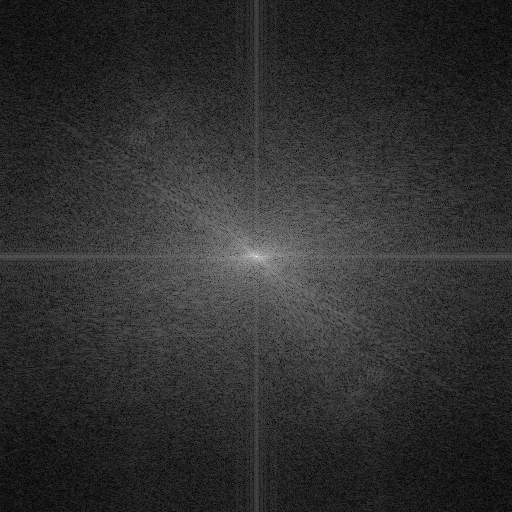
\includegraphics[width=\textwidth]{lena_fft}
        \caption{Frequency spectrum}
    \end{subfigure}
    \caption{Image before and after transformation by \fft}
\end{figure}

\section{Description of the implementation of the filters}
At the end of each filter there is a function called apply_mask_filter or apply_mask_filter_complex for complex numbers. Those functions are implemented before the filters, becuase they are responsible for applying the Fourier Transformation and saving processed images to the output files.
\subsection{Low-pass filter}
The low-pass filter 
\begin{lstlisting}
fn apply(&self, image: &mut RgbImage) {
        let radius_squared = self.radius * self.radius;
        let half_width = image.width() / 2;
        let half_height = image.height() / 2;
        let mask = move |x: u32, y: u32| {
            let x = u32::abs_diff(x, half_width);
            let y = u32::abs_diff(y, half_height);
            if x * x + y * y <= radius_squared {
                1.0
            } else {
                0.0
            }
        };
        apply_mask_filter::<FFT, _>(image, &mask);
    }
\end{lstlisting}
\subsection{High-pass filter}
\begin{lstlisting}
 fn apply(&self, image: &mut RgbImage) {
        let radius_squared = self.radius * self.radius;
        let half_width = image.width() / 2;
        let half_height = image.height() / 2;
        let mask = move |x: u32, y: u32| {
            let x = u32::abs_diff(x, half_width);
            let y = u32::abs_diff(y, half_height);
            if x * x + y * y > radius_squared {
                1.0
            } else {
                0.0
            }
        };
        apply_mask_filter::<FFT, _>(image, &mask);
    }
\end{lstlisting}
\subsection{Band-pass filter}
\begin{lstlisting}
 fn apply(&self, image: &mut RgbImage) {
        let from_squared = self.from_radius.pow(2);
        let to_squared = self.to_radius.pow(2);
        let half_width = image.width() / 2;
        let half_height = image.height() / 2;
        let mask = move |x: u32, y: u32| {
            let x = u32::abs_diff(x, half_width);
            let y = u32::abs_diff(y, half_height);
            let distance_squared = x*x + y*y;
            match (distance_squared.cmp(&from_squared), distance_squared.cmp(&to_squared)) {
                (Less, _) => 0.0,
                (_, Greater) => 0.0,
                (_,_) => 1.0
            }
        };
        apply_mask_filter::<FFT, _>(image, &mask);
    }
\end{lstlisting}
\subsection{Band-cut filter}
\begin{lstlisting}
 fn apply(&self, image: &mut RgbImage) {
        let from_squared = self.from_radius.pow(2);
        let to_squared = self.to_radius.pow(2);
        let half_width = image.width() / 2;
        let half_height = image.height() / 2;
        let mask = move |x: u32, y: u32| {
            let x = u32::abs_diff(x, half_width);
            let y = u32::abs_diff(y, half_height);
            let distance_squared = x*x + y*y;
            match (distance_squared.cmp(&from_squared), distance_squared.cmp(&to_squared)) {
                (Less, _) => 1.0,
                (_, Greater) => 1.0,
                (_,_) => 0.0
            }
        };
        apply_mask_filter::<FFT, _>(image, &mask);
    }
\end{lstlisting}
\subsection{High-pass filter with detection of edge direction filter}
\subsection{Phase modifying filter}
\begin{lstlisting}
 fn apply(&self, image: &mut RgbImage) {
        let height = image.height() as f64;
        let width = image.width() as f64;
        let mask = move |x: u32, y: u32| {
            Complex::exp(Complex::i() * (-1.0 * (x as f64 * self.k * 2.0 * std::f64::consts::PI) / height + -1.0 * (y as f64 * self.l * 2.0 * std::f64::consts::PI) / width + (self.k + self.l) * std::f64::consts::PI))
        };
        let mut image_clone = image.clone();
        apply_mask_filter_complex::<FFT, _>(&mut image_clone, &mask);
        *image = image_clone;
    }
\end{lstlisting}

\section{Analysis of the filtering results}
\subsection{Low-pass filter}
The result of running the low-pass filter on the sample image is presented below.
\begin{figure}[H]\centering
    \begin{subfigure}[t]{\subfiguresize}\centering
        \includegraphics[width=\textwidth]{img/lena.png}
        \caption{before}
    \end{subfigure}
    \hspace{2em}
    \begin{subfigure}[t]{\subfiguresize}\centering
        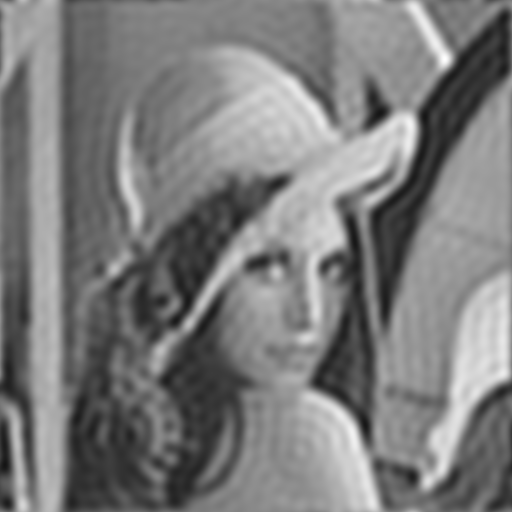
\includegraphics[width=\textwidth]{img/lena_lowpass.png}
        \caption{after}
    \end{subfigure}\\[1em]
    \caption{Results of applying low-pass filter}
\end{figure}   
\subsection{High-pass filter}
The result of running the high-pass filter on the sample image is presented below.
\begin{figure}[H]\centering
    \begin{subfigure}[t]{\subfiguresize}\centering
        \includegraphics[width=\textwidth]{img/lena.png}
        \caption{before}
    \end{subfigure}
    \hspace{2em}
    \begin{subfigure}[t]{\subfiguresize}\centering
        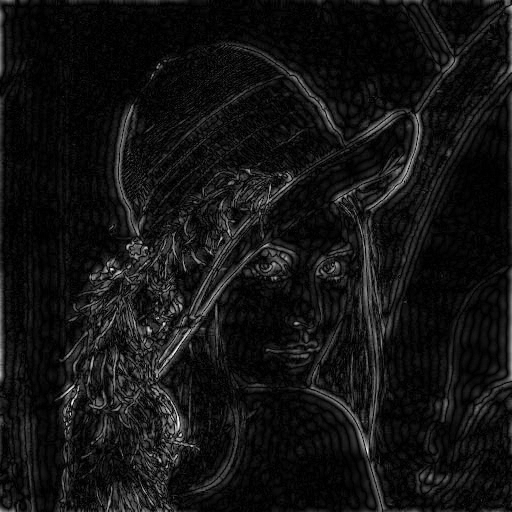
\includegraphics[width=\textwidth]{img/lena_highpass.png}
        \caption{after}
    \end{subfigure}\\[1em]
    \caption{Results of applying high-pass filter}
\end{figure}  
\subsection{Band-pass filter}
The result of running the band-pass filter on the sample image is presented below.
\begin{figure}[H]\centering
    \begin{subfigure}[t]{\subfiguresize}\centering
        \includegraphics[width=\textwidth]{img/lena.png}
        \caption{before}
    \end{subfigure}
    \hspace{2em}
    \begin{subfigure}[t]{\subfiguresize}\centering
        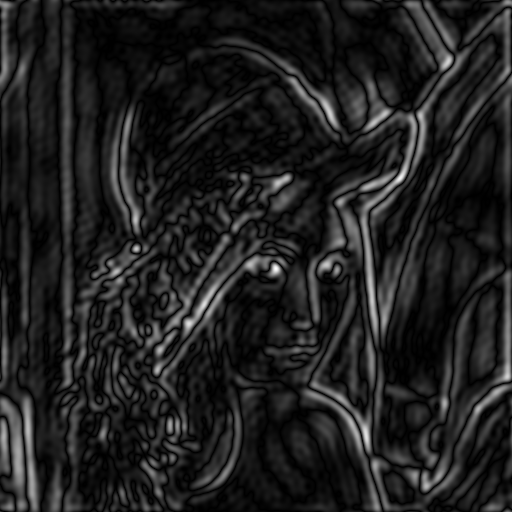
\includegraphics[width=\textwidth]{img/lena_bandpass.png}
        \caption{after}
    \end{subfigure}\\[1em]
    \caption{Results of applying band-pass filter}
\end{figure}  
\subsection{Band-cut filter}
The result of running the band-cut filter on the sample image is presented below.
\begin{figure}[H]\centering
    \begin{subfigure}[t]{\subfiguresize}\centering
        \includegraphics[width=\textwidth]{img/lena.png}
        \caption{before}
    \end{subfigure}
    \hspace{2em}
    \begin{subfigure}[t]{\subfiguresize}\centering
        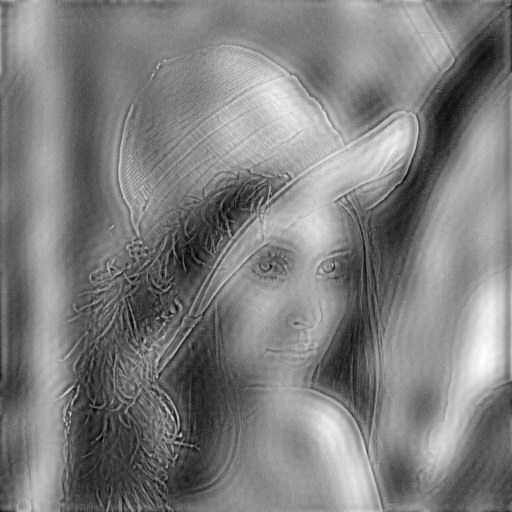
\includegraphics[width=\textwidth]{img/lena_bandcut.png}
        \caption{after}
    \end{subfigure}\\[1em]
    \caption{Results of applying band-cut filter}
\end{figure}  
\subsection{High-pass filter with detection of edge direction filter}
\subsection{Phase modifying filter}
 
\section{Description of other changes which took place in the application}

No additional changes took place in the application.

\vfill
\section*{Teacher's remarks}
\begin{tabularx}{\textwidth}{|X|}
    \hline
    \vspace{7cm}
    \phantom{.} \\
    \hline
\end{tabularx}

\end{document}